
\noindent 
\textbf{\stepcounter{zadatak}
\thecjelina.\thezadatak.}
Vanjska sila iznosa $F_0=50\ N$ djeluje na blok A mase $m_A= 5\ kg$ koji vuče blok B mase $m_B= 3\ kg$ (vidjeti skicu). 
\begin{enumerate}[label=\alph*)]
 \item Izračunajte iznos sile kojom blokovi djeluju jedan na drugoga ako pretpostavimo da nema trenja.
 \item Izračunajte iznos sile kojom blokovi djeluju jedan na drugoga kada je koeficijent kinetičkog trenja između blokova i podloge $\mu_k =0,3$.
\end{enumerate}


\begin{figure}[h]%{r}{0.7\textwidth} % Inline image example
  \begin{center}
    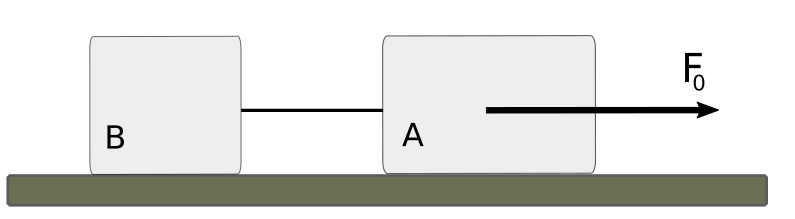
\includegraphics[scale=0.40]{../03_Dinamika_materijalne_tocke/Zadatak_D301.png}
  \end{center}
  %\caption{Fish}
\end{figure}

